\documentclass{JACoW-GSI-2015}

\usepackage{graphicx}
\usepackage[utf8]{inputenc}

\setlength{\titleblockheight}{35mm} % ??? Do we need that?

\begin{document}

\title{Time precision of the CBM RICH readout system}

\author[1]{E.~Ovcharenko\thanks{eovchar@jinr.ru}}
\author[1]{S.~Belogurov}
\author[2]{C.~Pauly}

\affil[1]{LIT JINR, Dubna, Russia}
\affil[2]{University of Wuppertal, Germany}

\maketitle

During a common CBM beam test at CERN-PS in Nov 2014 a CBM RICH prototype including a camera of 16 MAPMTs has been successfully tested. Details about the readout and DAQ system can be found in \cite{RICH2016, PEPANL}. There are two types of events in the data gathered during the beamtime. In both cases almost simultaneous hits are registered by multiple pixels of the photosensitive camera. The first type is a flash of a laser with $\approx$40~ps duration, which is one order of magnitude lower than the transition time spread in the MAPMT. The second type of events is formed by the hits from the Cherenkov photons of one charged particle. The time spread of arriving photons can be as high as 100~ps for Cherenkov rings and 70~ps for a laser flash due to the geometry of the setup. Analysis of such events after applying fine time calibration and inter-channel delay correction in software allows characterization of the time precision of the full readout system. 

It is impossible to measure the exact time of the photon arrival in the absolute time scale so the relative times are analysed. Consider all $N$ hits of one reconstructed event --- laser flash or Cherenkov ring. Each hit has a timestamp $t$ and the channel ID $c$. For hits with $c$ in some set $A_k$, $k \in [1,4]$ we build the time difference distribution as

{\centering
$t_i-t_j$, $i \in [1,N]$, $j \in [1,N]$, $i \neq j$. \\
}

By taking the same difference twice we make the distribution symmetrical. In order to characterize the time precision of the readout system in general and evaluate the contribution of its components, the studied area of the camera can be limited by filtering the hits from a specific subset of channels. Of particular interest are the following: ($A_1$)~one pair of channels, ($A_2$)~16~channels read out by one PADIWA FEB, ($A_3$)~64~channels of one MAPMT, ($A_4$)~256~channels of 4~MAPMTs. 

Timestamps in each channel fluctuate independently following similar probability distribution functions. Thus the measured width of this distribution is $\sqrt 2$ larger than the actual time precision. For a pair of channels, the FWHM of the distribution is 600~ps which corresponds to a time precision of 425~ps. This value is almost two times higher than the transition time spread of the MAPMT. There are two main reasons for that: instability of inter-channel delay corrections over time and absence of walk correction. In order to implement the walk correction procedure one needs to have stable time-over-threshold (ToT) measurements which are not available in the beamtime data.



%Results for laser flashes are shown in fig.~\ref{fig:TimeResEvolutionLaser}.
Table~\ref{tabl:EvolutionParams} shows the evolution of the RMS and FWHM with increasing the number of analysed channels. Note that for events with laser flashes the RMS almost does not change while the FWHM increases and the shape of the distribution gets closer to a Gaussian. This can be interpreted as smearing of the features of individual channels by averaging. For hits from one Cherenkov ring (see fig.~\ref{fig:TimeResEvolutionRings}) the FWHM and RMS increase with increasing number of analysed channels, but FWHM again goes up much faster than RMS.

\begin{table}[tbh]
\caption{FWHM and RMS of the time difference distributions for different analysed areas.}
\label{tabl:EvolutionParams}
\begin{tabular}{ | p{0.25\linewidth} | p{0.11\linewidth} | p{0.11\linewidth} | p{0.11\linewidth} | p{0.11\linewidth} | }
	\hline
	\scriptsize{Analysed area} & \scriptsize{Pair of channels} & \scriptsize{PADIWA FEB} & \scriptsize{One MAPMT} & \scriptsize{Four MAPMTs} \\
	\hline
	\scriptsize{Num. of channels} & 2 & 16 & 64 & 256 \\
	\hline
	\scriptsize{FWHM, laser, [ns]} & 1.1 & 1.2 & 1.5 & 1.7 \\
	\hline
	\scriptsize{FWHM, rings, [ns]} & 0.6 & 0.8 & 1.0 & 1.3 \\
	\hline
	\scriptsize{RMS, laser, [ns]} & 0.913 & 1.093 & 0.997 & 1.034 \\
	\hline
	\scriptsize{RMS, rings, [ns]} & 1.238 & 1.379 & 1.430 & 1.487 \\
	\hline
	\scriptsize{Color on fig.~\ref{fig:TimeResEvolutionRings}} & blue & red & green & black \\
	\hline
\end{tabular}
\end{table}

%\begin{figure}[tbh]
%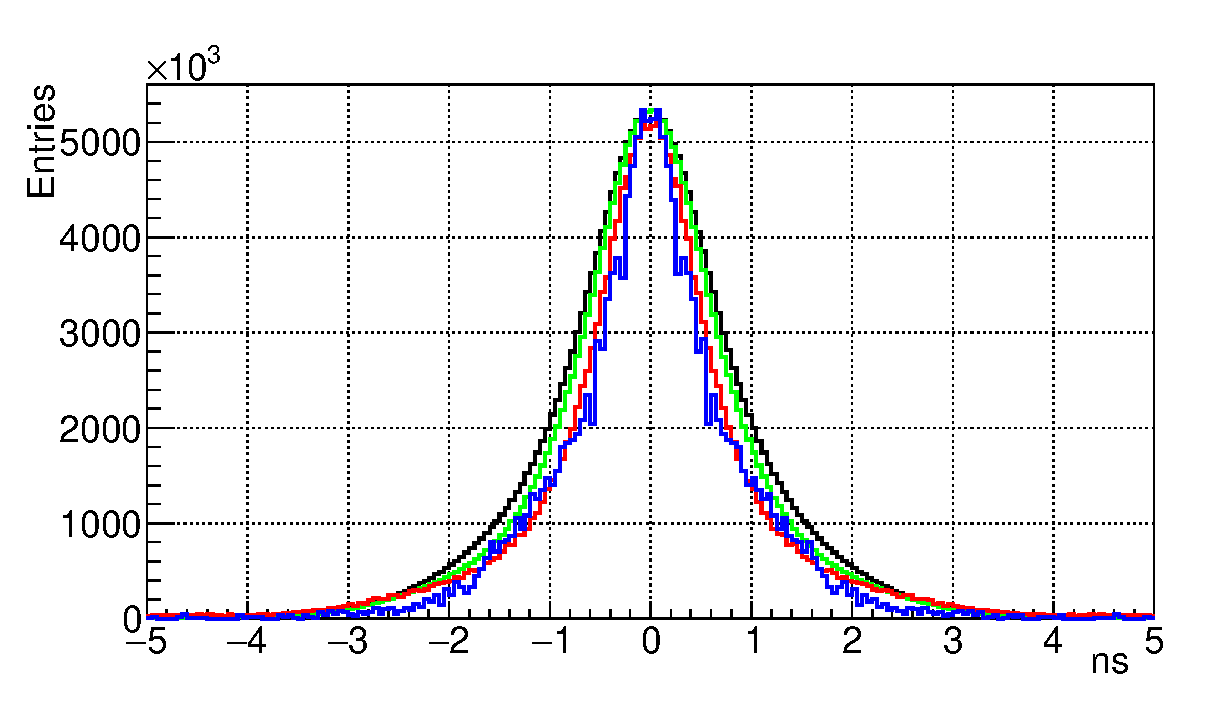
\includegraphics[width=0.8\linewidth]{../PTE/pictures/24_TimePrecision_evolution_laser_feb2017.eps}
%\caption{Distributions for 4 different sets of channels for events with laser flashes.}
%\label{fig:TimeResEvolutionLaser}
%\end{figure}

\begin{figure}[tbh]
\centering
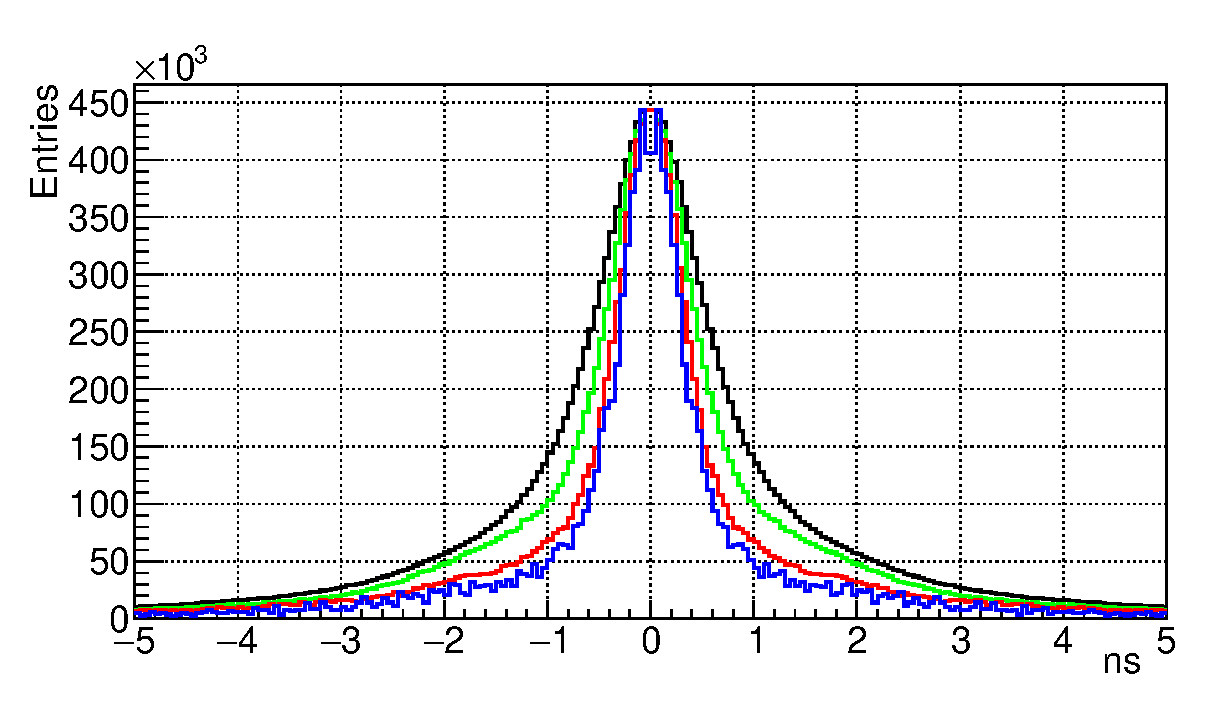
\includegraphics[width=0.9\linewidth]{../PTE/pictures/25_TimePrecision_evolution_rings_feb2017.eps}
\caption{Time difference distributions for 4 different sets of channels for events with Cherenkov rings.}
\label{fig:TimeResEvolutionRings}
\end{figure}

\begin{thebibliography}{9}

\bibitem{RICH2016}
E.~Ovcharenko et~al. //
Development of the CBM RICH readout electronics and DAQ,
RICH2016 proceedings,
Submitted to NIM A

\bibitem{PEPANL}
E.~Ovcharenko et~al. //
Tests of the CBM RICH readout and DAQ prototype,
Submitted to PEPAN letters

\end{thebibliography}

\end{document}